\usetikzlibrary{calc}

\begin{figure}[H]
\centering
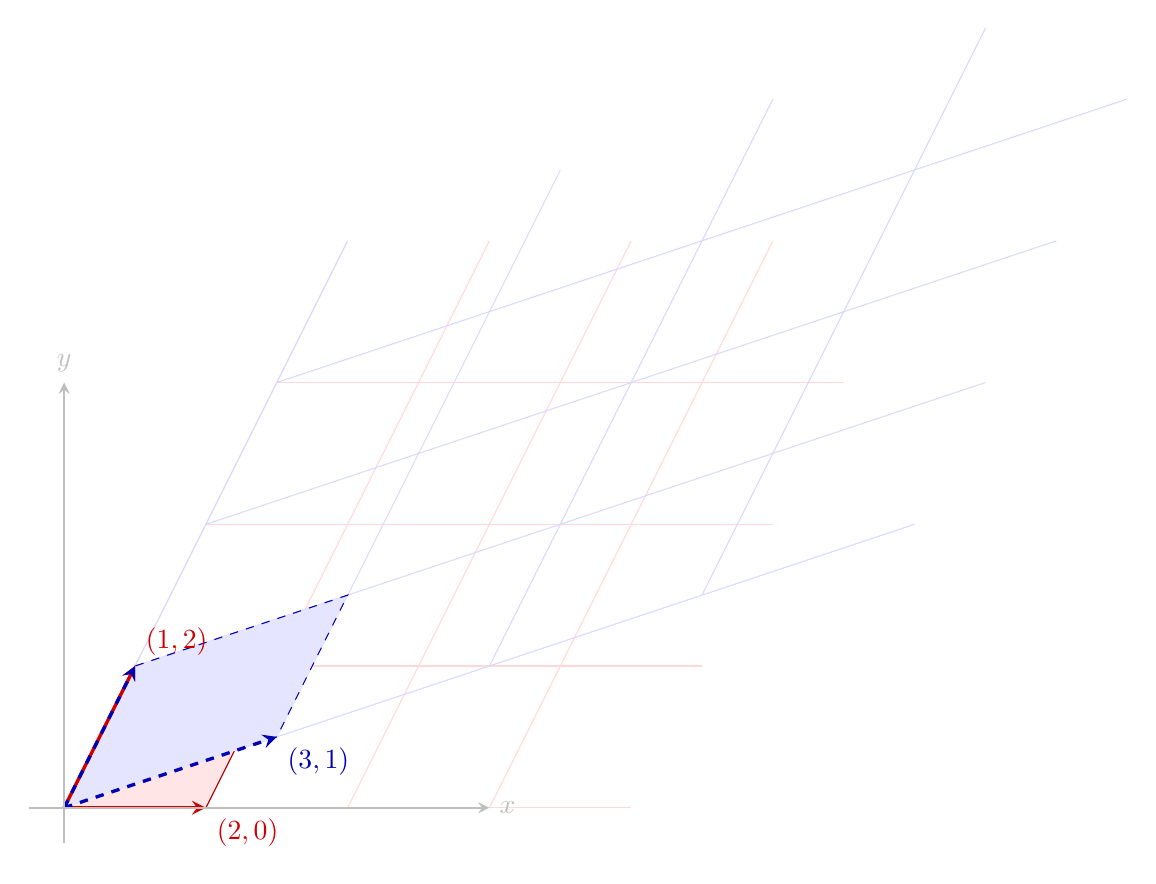
\begin{tikzpicture}[scale=0.9, >=stealth]

    % ====== Define columns for A1 ======
    \def\aOne{2} % first vector of A1
    \def\bOne{0}
    \def\cOne{1} % second vector of A1
    \def\dOne{2}

    % ====== Define columns for A2 ======
    \def\aTwo{3}
    \def\bTwo{1}
    \def\cTwo{1}
    \def\dTwo{2}

    % ===== Original Grid (A1) =====
    \foreach \i in {0,1,2,3} {
        % Lines parallel to v1 (shifted by multiples of v2)
        \draw[red!15, thin] ({\i*\cOne},{\i*\dOne}) -- ({\i*\cOne + 4*\aOne},{\i*\dOne + 4*\bOne});
    }
    \foreach \j in {0,1,2,3} {
        % Lines parallel to v2 (shifted by multiples of v1)
        \draw[red!15, thin] ({\j*\aOne},{\j*\bOne}) -- ({\j*\aOne + 4*\cOne},{\j*\bOne + 4*\dOne});
    }

    % ===== New Grid (A2) =====
    \foreach \i in {0,1,2,3} {
        \draw[blue!15, thin] ({\i*\cTwo},{\i*\dTwo}) -- ({\i*\cTwo + 4*\aTwo},{\i*\dTwo + 4*\bTwo});
    }
    \foreach \j in {0,1,2,3} {
        \draw[blue!15, thin] ({\j*\aTwo},{\j*\bTwo}) -- ({\j*\aTwo + 4*\cTwo},{\j*\bTwo + 4*\dTwo});
    }

    % ===== Parallelograms =====
    \filldraw[fill=red!10, draw=red!70!black]
        (0,0) -- (\aOne,\bOne) -- ({\aOne+\cOne},{\bOne+\dOne}) -- (\cOne,\dOne) -- cycle;
    \filldraw[fill=blue!10, draw=blue!70!black, dashed]
        (0,0) -- (\aTwo,\bTwo) -- ({\aTwo+\cTwo},{\bTwo+\dTwo}) -- (\cTwo,\dTwo) -- cycle;

    % ===== Vectors =====
    \draw[->,very thick,red!80!black] (0,0) -- (\aOne,\bOne) node[below right] {$(2,0)$};
    \draw[->,very thick,red!80!black] (0,0) -- (\cOne,\dOne) node[above right] {$(1,2)$};
    \draw[->,very thick,blue!70!black,dashed] (0,0) -- (\aTwo,\bTwo) node[below right] {$(3,1)$};
    \draw[->,very thick,blue!70!black,dashed] (0,0) -- (\cTwo,\dTwo);

    % ===== Axes (optional) =====
    \draw[->,thick,gray!50] (-0.5,0) -- (6,0) node[right] {$x$};
    \draw[->,thick,gray!50] (0,-0.5) -- (0,6) node[above] {$y$};

\end{tikzpicture}
\caption{Comparing the new transformation}
\end{figure}
